%        File: CommReport.tex
%     Created: 日 9月 22 03:00 下午 2019 C
% Last Change: 日 9月 22 03:00 下午 2019 C
%
\documentclass[12pt]{utils/mydoc}
\usepackage{graphicx}
\usepackage[dvipsnames]{xcolor}
\usepackage{wrapfig}
\usepackage{enumerate}
\usepackage{amsmath,mathrsfs,amsfonts}
\usepackage{booktabs}
\usepackage{tabularx}
\usepackage{colortbl}
\usepackage{multirow,makecell}
\usepackage{multicol}
\usepackage{ulem} % \uline
\usepackage{listings}
\usepackage{tikz}
\usepackage{tcolorbox}
\usepackage{fontawesome}
\usepackage{cite}

% \CTEXoptions[today=old] % use en-Us date

\title{\bfseries \sffamily Meeting Report}
\date{September 25, 2019} % clear date info

\begin{document}
\maketitle

This report is mainly talking about the academic communication with 
Prof. YanLin Geng at Sunday, September 22, 2019.

\section{Some variations of GANs}

In this section we will introduce some variations of GANs.

\subsection{InfoGAN}

The InfoGAN\cite{Chen2016InfoGAN} bind information theory to GANs.

\begin{abstract}
  This paper describes InfoGAN, an information-theoretic extension to the Generative 
  Adversarial Network that is able to learn disentangled representations in a
  completely unsupervised manner. InfoGAN is a generative adversarial network
  that also maximizes the mutual information between a small subset of the latent
  variables and the observation. We derive a lower bound of the mutual information
  objective that can be optimized efficiently. Specifically, InfoGAN successfully
  disentangles writing styles from digit shapes on the MNIST dataset, pose from
  lighting of 3D rendered images, and background digits from the central digit on
  the SVHN dataset. It also discovers visual concepts that include hair styles, 
  presence/absence of eyeglasses, and emotions on the CelebA face dataset. Experiments
  show that InfoGAN learns interpretable representations that are competitive with
  representations learned by existing supervised methods.
\end{abstract}

\begin{description}
  \item[Problems] The vanilla GAN imposes no restriction on input noise $z$, thus learns
    highly entangled representations.
  \item[Methods] Decompose the input noise into two parts: 1) incompressible noise; 2) 
    latent code.
  \item[Contributions] Provides more interpretability by introducing latent codes on input
    noise; learns disentangled representations in a completely unsupervised manner. 
\end{description}

\subsection{SS-InfoGAN}

The ss-InfoGAN\cite{spurr2017guiding} use a relatively small amount of labels to guide the 
training of InfoGAN.

\begin{abstract}
  In this paper we propose a new semi-supervised GAN architecture
  (ss-InfoGAN) for image synthesis that leverages information from few labels (as
  little as 0.2\%, max. 10\% of the dataset) to learn semantically meaningful and
  controllable data representations where latent variables correspond to label 
  categories. The architecture builds on Information Maximizing Generative 
  Adversarial Networks (InfoGAN) and is shown to learn both continuous and 
  categorical codes and achieves higher quality of synthetic samples compared to
  fully unsupervised settings. Furthermore, we show that using small amounts of 
  labeled data speeds-up training convergence. The architecture maintains the 
  ability to disentangle latent variables for which no labels are available. 
  Finally, we contribute an information-theoretic reasoning on how introducing 
  semi-supervision increases mutual information between synthetic and real data.  
\end{abstract}

\begin{figure}[hpb!]
  \centering
  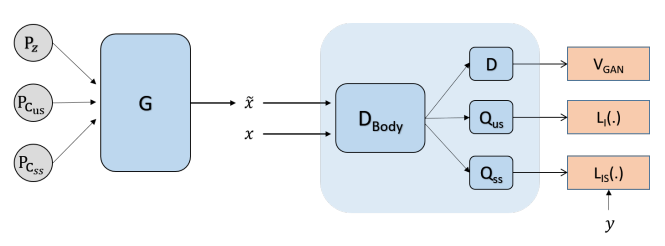
\includegraphics[width=0.6\textwidth]{figss/ss-infogan.png}
  \caption{Architecture of ss-InfoGAN}
  \label{fig:}
\end{figure}

\begin{description}
  \item[Problems] InfoGAN\cite{Chen2016InfoGAN} have recently been shown to learn disentangled
    representations, yet the extracted representations are not always directly interpretable
    by humans and lack direct measures of control due to the unsupervised training scheme.
  \item[Methods] Leverage information from few labels, by decomposing latent code into two parts:
    unsupervised and supervised. Direct training to increase $I(C_{ss}; X)$ and 
    $I(C_{ss}; \tilde{X})$, result in the increase of $I(X; \tilde{X})$.
  \item[Contributions] Achieve higher quality of synthetic samples compared to fully unsupervised
    settings; faster convergence rate than InfoGAN.
\end{description}

\subsection{SemiGAN}

The SemiGAN\cite{odena2016semi} is an extension of semi-supervised learning of GAN. 

\begin{abstract}
  We extend Generative Adversarial Networks (GANs) to the semi-supervised 
  context by forcing the discriminator network to output class labels. We
  train a generative model $G$ and a discriminator $D$ on a dataset with inputs
  belonging to one of $N$ classes. At training time, $D$ is made to predict 
  which of $N+1$ classes the input belongs to, where an extra class is added
  to correspond to the outputs of $G$. We show that this method can be used
  to create a more data-efficient classifier and that it allows for 
  generating higher quality samples than a regular GAN.
\end{abstract}

\begin{description}
  \item[Problems] The vanilla GAN is suitable for classification, and how the generator $G$, discriminator $D$ and classifier $C$ will affect each other.
  \item[Methods] Use softmax instead of sigmoid.
  \item[Innovations] ~
    \begin{itemize}
      \item Use GANs in semi-supervised classification.
      \item Better performance than CNN on some datasets.
      \item Faster training and better outputs of generator.
    \end{itemize}
  \item[Future work] Use ladder network for $D$ and $G$.
\end{description}

\subsection{CGAN}

The CGAN\cite{mirza2014conditional} proposes a conditional version of GAN.

\begin{abstract}
  Generative Adversarial Nets were recently introduced as a novel way to train
  generative models. In this work we introduce the conditional version of generative
  adversarial nets, which can be constructed by simply feeding the data, $y$, we wish
  to condition on to both the generator and discriminator. We show that this model
  can generate MNIST digits conditioned on class labels. We also illustrate how
  this model could be used to learn a multi-modal model, and provide preliminary
  examples of an application to image tagging in which we demonstrate how this
  approach can generate descriptive tags which are not part of training labels.
\end{abstract}

\begin{description}
  \item[Problems] Vanilla GAN can not generate a specific class of samples we want; vanilla GAN
    is not scalable for big amount of data categories; plenty of works focus on one-to-one
    mapping, however, one-to-many (e.g., image labeling) is also a common problem.
  \item[Methods] Feed label information into generator $G$ and discriminator $D$.
  \item[Innovations] Better control of generated images; generate tags that are not contained
    in training set.
  \item[Known cons] Network model is too simple; only one label for training.
  \item[Future work] Use more complicated network, add more than one label in training.
\end{description}

\subsection{CatGAN}

The CatGAN\cite{springenberg2015unsupervised} proposes a method for learning a classifier
based on unlabeled or partially labeled data.

\begin{abstract}
  In this paper we present a method for learning a discriminative classifier from
  unlabeled or partially labeled data. Our approach is based on an objective function
  that trades-off mutual information between observed examples and their predicted
  categorical class distribution, against robustness of the classifier to an adversarial
  generative model. The resulting algorithm can either be interpreted as a natural
  generalization of the generative adversarial networks (GAN) framework or as an
  extension of the regularized information maximization (RIM) framework to robust
  classification against an optimal adversary. We empirically evaluate our method
  – which we dub categorical generative adversarial networks (or CatGAN) – on
  synthetic data as well as on challenging image classification tasks, demonstrating
  the robustness of the learned classifiers. We further qualitatively assess the fidelity
  of samples generated by the adversarial generator that is learned alongside the
  discriminative classifier, and identify links between the CatGAN objective and
  discriminative clustering algorithms (such as RIM).
\end{abstract}

\begin{description}
  \item[Problems] Existing methods for semi-supervised or unsupervised learning (e.g.,
    Gaussian mixture model, K-means, Maximum margin clustering (MMC), RIM, Boltzman 
    machines, autoencoders) overfit when sample distribution is far from real distribution.
  \item[Methods] Combining both the generative and the discriminative perspective, 
    learn discriminative neural network classifiers $D$ that maximize mutual information (MI) 
    between the inputs $x$ and the labels $y$ (as predicted through the conditional 
    distribution $p(y|x, D))$ for a number of $K$ unknown categories.
  \item[Contributions] Introduce MI between observed data $x$ and predicted label $y$ in
    loss function; provide robustness for RIM.
  \item[Future work] Introduce Laplacian pyramids.
\end{description}

\subsection{BiGAN}

The BiGAN\cite{donahue2016adversarial} learns a generation network and an inference
network using an adversarial process.

\begin{abstract}
  The ability of the Generative Adversarial Networks (GANs) framework to learn
  generative models mapping from simple latent distributions to arbitrarily complex
  data distributions has been demonstrated empirically, with compelling results
  showing that the latent space of such generators captures semantic variation in
  the data distribution. Intuitively, models trained to predict these semantic latent
  representations given data may serve as useful feature representations for auxiliary
  problems where semantics are relevant. However, in their existing form, GANs
  have no means of learning the inverse mapping – projecting data back into the
  latent space. We propose Bidirectional Generative Adversarial Networks (BiGANs)
  as a means of learning this inverse mapping, and demonstrate that the resulting
  learned feature representation is useful for auxiliary supervised discrimination tasks,
  competitive with contemporary approaches to unsupervised and self-supervised
  feature learning.
\end{abstract}

\begin{figure}[htb]
  \centering
  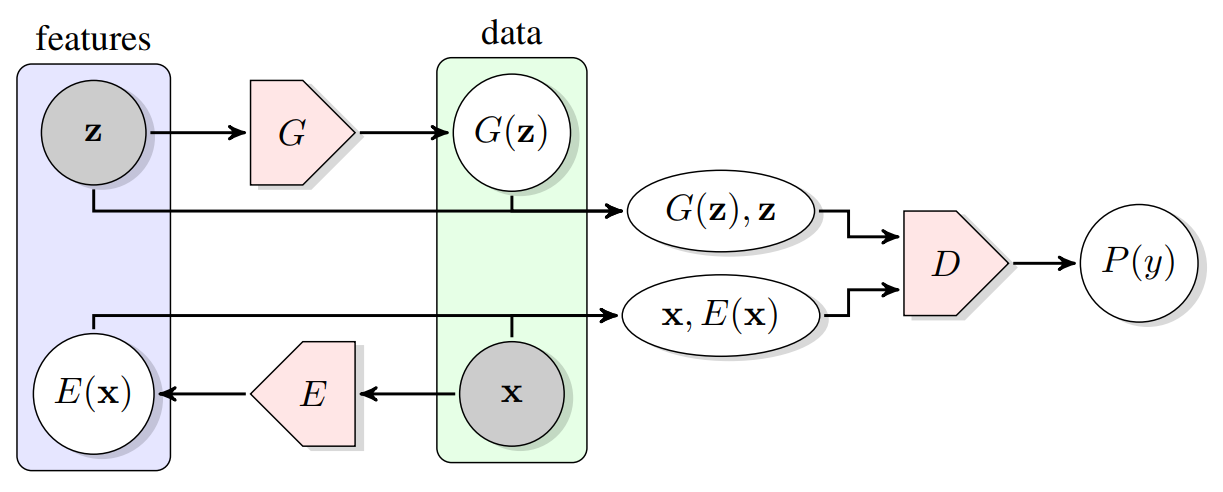
\includegraphics[width=0.7\textwidth]{figss/ali.png}
  \caption{The structure of Bidirectional Generative Adversarial Networks (BiGAN).}
  \label{fig:}
\end{figure}

\begin{description}
  \item[Problems] Generators of GAN map noise to sample, but unable to do the inverse.
  \item[Contributions] Not only generating, but also encoding; the learning of the
    encoder is an auxiliary for the main task.
\end{description}

\subsection{ACGAN}

The ACGAN\cite{odena2017conditional} improves the performance of generated samples of GANs.

\begin{abstract}
  In this paper we introduce new methods for the improved training of generative 
  adversarial networks (GANs) for image synthesis. We construct a variant of GANs
  employing label conditioning that results in $128 \times 128$ resolution image samples
  exhibiting global coherence. We expand on previous work for image quality 
  assessment to provide two new analyses for assessing the discriminability and 
  diversity of samples from class-conditional image synthesis models.  These 
  analyses demonstrate that high resolution samples provide class information 
  not present in low resolution samples. Across 1000 ImageNet classes, $128 \times 128$
  samples are more than twice as discriminable as artificially resized $32 \times 32$
  samples. In addition, 84.7\% of the classes have samples exhibiting diversity 
  comparable to real ImageNet data.
\end{abstract}

\begin{description}
  \item[Problems] Transform a $32 \times 32$ picture to $128 \times 128$ will result in
    blur on picture. Models is not very good if GANs generate only one samples for each
    class.
  \item[Methods] Use inception accuracy and MS-SSIM (Multi-Scale Structural Similarity
    for IMage quality assessment) to assess generated samples.
  \item[Innovations] Measurement of synthetic images and crash of GAN.
\end{description}

\subsection{CVAE-GAN}

The CVAE-GAN\cite{bao2017cvae} is a general learning framework that combines
VAE and GAN.

\begin{abstract}
  We present variational generative adversarial networks,
  a general learning framework that combines a variational
  auto-encoder with a generative adversarial network, for
  synthesizing images in fine-grained categories, such as
  faces of a specific person or objects in a category. Our
  approach models an image as a composition of label and
  latent attributes in a probabilistic model. By varying the
  fine-grained category label fed into the resulting generative
  model, we can generate images in a specific category with
  randomly drawn values on a latent attribute vector. Our
  approach has two novel aspects. First, we adopt a cross entropy 
  loss for the discriminative and classifier network, but
  a mean discrepancy objective for the generative network.
  This kind of asymmetric loss function makes the GAN training 
  more stable. Second, we adopt an encoder network to
  learn the relationship between the latent space and the real
  image space, and use pairwise feature matching to keep the
  structure of generated images. We experiment with natural
  images of faces, flowers, and birds, and demonstrate that
  the proposed models are capable of generating realistic and
  diverse samples with fine-grained category labels. We further 
  show that our models can be applied to other tasks,
  such as image inpainting, super-resolution, and data 
  augmentation for training better face recognition models.
\end{abstract}

\begin{description}
  \item[Problems] It is difficult for generative model to capture the underlying
    data distribution since a collection of image samples may lie on a very
    complex manifold. Also, what is we want to generate images of fine-grained
    object categories?
  \item[Methods] Combine CVAE and GAN.
  \item[Innovations] ~
    \begin{itemize}
      \item Change generator loss to average divergence, thus stabilizing the training.
      \item Use encoder thus generating better images.
      \item Contributes to image inpainting, images rotate and data augmentation.
    \end{itemize}
\end{description}

\section{Other works}

\begin{description}
  \item[LiKun Cai] Derive a new GAN objective using Renyi Divergence.
  \item[Kai Liang] Deep learning (DL) theory: why that simple SGD (Stochastic Gradient
    Descent) do work in DL? From three perspective: 1) Generalization; 2) Optimization;
    3) Approximation.
\end{description}

\section{From Prof. Geng}

These may be Prof. Geng's research interests.

\begin{enumerate}
  \item Convergence and reachability of multi-user channels.
  \item Random code may work powered by today's computation ability, is there any mathematical
    principle hidden in it?
  \item Can multi-letter random code degenerate to single-letter case, is there any structure
    in it?
  \item Assessment of outputs of generator in GAN.
  \item Like data which can be compressed, is it possible for network structure?
\end{enumerate}

%\bibliographystyle{plain}
\bibliographystyle{ieeetr}
\bibliography{CommReport.bib}

\end{document}
